\chapter{L’Univers newtonien en expansion}

\lectureoverview{La cosmologie moderne commence lorsque l’Univers lui-même est considéré comme un système physique. En partant de l’isotropie et de l’homogénéité à grande échelle, nous introduisons un réseau comobile et décrivons son mouvement au moyen d’un unique facteur d’échelle \(a(t)\). Le théorème des coquilles de Newton ramène alors le problème gravitationnel à plusieurs corps à une équation pour \(a(t)\). La conservation de l’énergie distingue les Univers qui se recontractent, l’Univers critique et ceux qui s’étendent éternellement ; dans le cas critique dominé par la matière, on obtient la première équation de Friedmann et la loi \(a(t)\propto t^{2/3}\).}

\section{Quand la cosmologie est devenue une physique}

La cosmologie est une discipline ancienne, mais la cosmologie quantitative est récente. Pour ce qui nous occupe ici, il n’est pas nécessaire de commencer par les Grecs. Les repères historiques utiles sont la découverte de l’expansion cosmique par Hubble au deuxième quart du vingtième siècle, puis la reconnaissance du fond diffus de micro-ondes, à environ trois kelvins, comme vestige d’un Univers primordial chaud.

Avant que les mesures ne deviennent précises, l’astronomie ressemblait nécessairement en grande partie à l’histoire naturelle. On découvrait une étoile inhabituelle, classait une galaxie singulière, mesurait ce qui pouvait l’être et dressait un catalogue d’objets. Ces objets étaient bien sûr des systèmes physiques : ils possédaient un moment cinétique, contenaient des éléments chimiques et obéissaient aux lois de la mécanique. Le changement décisif a consisté à traiter \emph{l’Univers entier} comme un seul système physique, régi par des équations suffisamment précises pour être confrontées aux observations.

C’est le sujet de ce chapitre. Nous ne nous contenterons pas d’énumérer le contenu de l’Univers ; nous chercherons à en déterminer les variables, le mouvement et la loi dynamique. Les équations ne sont pas un ornement que l’on ajoute après la cosmologie. Elles permettent de faire de l’Univers un problème de physique.

Historiquement, l’Univers en expansion a été compris dans le cadre de la relativité générale. Logiquement, toutefois, une grande partie du raisonnement initial est newtonienne. Un physicien du dix-septième siècle qui aurait deviné le bon mouvement à grande échelle aurait pu dériver un modèle remarquablement satisfaisant. Commencer par Newton ne vise pas à remplacer la relativité, mais à mettre au jour la mécanique que la relativité réorganisera ensuite sous une forme géométrique.

\section{Isotropie, homogénéité et principe cosmologique}

La première étape relève de l’observation. À suffisamment grande échelle, l’Univers est approximativement \emph{isotrope} : après avoir moyenné sur des régions du ciel et regardé au-delà de l’avant-plan de la Voie lactée, il paraît semblable dans toutes les directions. Cela ne signifie pas qu’il soit rigoureusement uniforme. Il y a une différence entre regarder directement une étoile proche et observer une région vide, et la répartition de la matière comporte de véritables structures. L’isotropie est une propriété moyennée à grande échelle.

L’homogénéité est une affirmation différente. Elle signifie que l’Univers moyenné est identique d’un lieu à l’autre. Un observateur situé à plusieurs galaxies de nous devrait voir, après le même moyennage à grande échelle, approximativement le même type d’Univers que nous.

Dans une première approximation, une galaxie peut être traitée comme un simple point matériel. L’Univers visible contient environ
\begin{equation}
N_{\rm gal}\sim 10^{11}
\end{equation}
galaxies, comptant chacune de l’ordre de \(10^{11}\) étoiles. Cela représente environ \(10^{22}\) étoiles. Si l’on prend dix planètes par étoile comme estimation délibérément grossière de l’ordre de grandeur, on obtient \(10^{23}\) planètes, ce qui est, de façon amusante, proche d’une mole de planètes. Cette estimation numérique n’intervient pas dans la dynamique, mais elle fixe l’échelle du système idéalisé.

\begin{classroomqa}
\classquestion{Quel est, à un ordre de grandeur près, le nombre de galaxies dans l’Univers observable ?}
\lecturerresponse{Environ cent milliards, soit \(10^{11}\). Avec environ \(10^{11}\) étoiles par galaxie, cela représente approximativement \(10^{22}\) étoiles dans l’Univers visible. Ces estimations d’échelle sont utiles à garder à l’esprit, même si le calcul qui suit remplace chaque galaxie par un seul point matériel. \lecturetimestamp{00:06:08--00:07:05}}
\end{classroomqa}

Pourquoi l’isotropie autour de nous suggère-t-elle l’homogénéité ? Imaginons une distribution isotrope qui ne soit \emph{pas} homogène. Sa densité devrait varier avec la distance à notre position, tout en restant indépendante de la direction : elle formerait en quelque sorte des coquilles concentriques autour de nous. Un observateur décalé par rapport au centre commun ne verrait plus une distribution isotrope. Il y a donc deux possibilités :
\begin{enumerate}
\item nous occupons un centre privilégié autour duquel l’Univers a été organisé ; ou
\item la répartition à grande échelle est approximativement homogène, de sorte qu’aucun point occupé n’est privilégié.
\end{enumerate}
La seconde possibilité est la plus parcimonieuse. L’isotropie, associée au refus de nous attribuer une position cosmique privilégiée, conduit à l’homogénéité.

\begin{classroomqa}
\classquestion{Quelle forme pourrait prendre une distribution isotrope mais inhomogène ?}
\lecturerresponse{Sa variation pourrait dépendre uniquement de la distance à notre position, formant une structure en coquilles centrée sur nous. Si l’observateur s’éloigne de ce centre, la distribution cesse d’être isotrope. À moins que notre position ne soit particulière, l’isotropie indique donc l’homogénéité. \lecturetimestamp{00:07:06--00:08:54}}
\end{classroomqa}

L’hypothèse qui combine ces deux propriétés s’appelle le \emph{principe cosmologique} : à suffisamment grande échelle, l’Univers est homogène et isotrope dans l’espace. Le qualifier de principe ne le prouve pas. Historiquement, les cosmologistes ont adopté cette hypothèse avant que les observations ne la justifient solidement. Elle doit son statut à sa réussite empirique.

L’homogénéité n’est pas non plus exacte. Les galaxies forment des amas et des superamas, et l’on a depuis longtemps discuté de structures s’étendant sur de très grandes fractions du ciel visible. Il convient plutôt d’affirmer que les fluctuations s’annulent par moyennage lorsque la région considérée est suffisamment grande---de l’ordre de centaines de millions à environ un milliard d’années-lumière dans cette introduction. Les observations peuvent affiner cette échelle ; la méthode consiste à lisser la description jusqu’à ce que les structures locales cessent de la dominer.

\begin{classroomqa}
\audiencequestion{L’uniformité du fond diffus cosmologique apporte-t-elle des éléments en faveur du principe cosmologique ?}
\lecturerresponse{Oui. Le principe cosmologique a été proposé avant que les observations ne le justifient solidement, mais le fond diffus a ensuite montré que l’Univers primordial était extraordinairement lisse. Les galaxies et les amas se sont formés à partir de faibles écarts par rapport à cet état lisse ; ils n’effacent pas les indices de son uniformité à grande échelle. \lecturetimestamp{00:10:53--00:11:43}}
\end{classroomqa}

\section{Un réseau qui se déplace avec les galaxies}

Une fois choisie cette approximation observationnelle, il faut choisir les variables. À la question « Quelle est la première étape dans la formulation d’un problème de physique ? », une réponse donnée en cours pourrait être : connaître les variables ; la réponse traditionnelle est : bien tailler son crayon. Ici, le choix judicieux des coordonnées permet de trouver la variable importante.

Imaginons un réseau tridimensionnel portant les étiquettes \(x,y,z\). Ces étiquettes ne sont pas nécessairement des distances mesurées en mètres : ce sont des nombres de coordonnées. Choisissons le réseau de telle sorte que, une fois moyennés les petits mouvements particuliers, chaque galaxie reste à un point fixe du réseau. Les galaxies sont alors \emph{comobiles}.

Un tel choix serait inutile si les galaxies se déplaçaient au hasard. Or les observations révèlent un mouvement cohérent à grande échelle. Les cellules voisines du réseau peuvent se dilater ou se contracter, mais la même dilatation ou contraction se produit partout. Toutes les distances physiques peuvent donc s’écrire comme le produit d’une même échelle dépendant du temps par une séparation fixe en coordonnées.

Pour deux galaxies \(A\) et \(B\),
\begin{equation}
\begin{aligned}
d_{AB}(t)&=a(t)\,\Delta\chi_{AB},\\
\Delta\chi_{AB}
&=\sqrt{(x_A-x_B)^2+(y_A-y_B)^2+(z_A-z_B)^2}.
\end{aligned}
\label{eq:c01-physical-distance}
\end{equation}
Si elles ne diffèrent que selon la coordonnée \(x\), cela se réduit à
\begin{equation}
d_{AB}(t)=a(t)\,\Delta x_{AB}.
\end{equation}
La fonction \(a(t)\) est le \emph{facteur d’échelle}. Sa normalisation absolue est conventionnelle : multiplier toutes les coordonnées comobiles par une constante et diviser \(a\) par la même constante ne change aucune distance physique. Les rapports comme \(a(t_2)/a(t_1)\) et les dérivées divisées par \(a\) contiennent l’information physique.

Dérivons l’équation~\eqref{eq:c01-physical-distance}. La séparation comobile étant fixe, on a
\begin{equation}
v_{AB}=\dot a\sqrt{(\Delta x)^2+(\Delta y)^2+(\Delta z)^2}.
\end{equation}
En divisant par la distance physique, on obtient
\begin{equation}
\frac{v_{AB}}{d_{AB}}=\frac{\dot a}{a}\equiv H(t),
\label{eq:c01-hubble-parameter}
\end{equation}
soit
\begin{equation}
\boxed{v_{AB}=H(t)d_{AB}.}
\label{eq:c01-hubble-law}
\end{equation}
C’est la loi de Hubble pour un écoulement idéalement homogène.

L’expression « constante de Hubble » peut induire en erreur. À un instant cosmique donné, la même valeur de \(H\) s’applique en tout lieu dans le modèle homogène, mais \(H(t)\) varie généralement au cours du temps. L’universalité spatiale n’implique pas la constance temporelle.

\begin{classroomqa}
\audiencequestion{En écrivant chaque distance comme le produit d’un même facteur \(a(t)\) par une séparation fixe en coordonnées, avons-nous déjà supposé la loi de Hubble ?}
\lecturerresponse{L’ansatz est certainement motivé par l’observation de Hubble ; sans indices d’une récession cohérente, on ne l’aurait pas imaginé. Son intérêt est d’organiser ces observations. Au lieu d’attribuer une vitesse indépendante à chaque galaxie, on décrit un unique réseau en expansion. Une fois cette description adoptée, la proportionnalité \(v=Hd\) découle de la dérivation. \lecturetimestamp{00:24:20--00:25:33}}
\end{classroomqa}

On peut décrire le même mouvement de deux façons. On peut dire que les galaxies s’éloignent les unes des autres dans l’espace, ou qu’elles restent à des positions comobiles fixes tandis que le réseau---et donc l’espace physique qui les sépare---se dilate. À ce stade, ce sont deux descriptions en coordonnées d’un même formalisme mathématique. La relativité générale rendra particulièrement naturelle l’idée d’un espace en expansion, mais aucune observation ne peut distinguer deux descriptions qui attribuent les mêmes séparations physiques à chaque instant.

\section{Bilan de masse dans une cellule comobile}

Avant d’introduire la gravitation, faisons le bilan de masse. Considérons une petite cellule de coordonnées de volume
\begin{equation}
\Delta V_{\rm com}=\Delta x\,\Delta y\,\Delta z.
\end{equation}
Elle doit néanmoins être assez grande pour contenir de nombreuses galaxies, afin que l’on puisse moyenner les fluctuations locales. Notons \(\nu\) la masse par unité de volume en coordonnées comobiles. La masse contenue dans la cellule est
\begin{equation}
\Delta M=\nu\,\Delta x\,\Delta y\,\Delta z.
\label{eq:c01-comoving-mass}
\end{equation}
Comme la cellule se déplace avec la matière, aucune galaxie ne traverse sa frontière dans l’écoulement idéal, et \(\Delta M\) reste constante.

Chaque arête physique est plus longue que l’arête correspondante en coordonnées d’un facteur \(a(t)\). Le volume physique est donc
\begin{equation}
\Delta V_{\rm phys}=a^3(t)\,\Delta x\,\Delta y\,\Delta z.
\end{equation}
La masse volumique physique est
\begin{equation}
\boxed{\rho(t)=\frac{\Delta M}{\Delta V_{\rm phys}}=\frac{\nu}{a^3(t)}.}
\label{eq:c01-density-dilution}
\end{equation}
La dilatation dilue la matière sans pression selon \(a^{-3}\) ; la contraction la concentre suivant la même loi.

Jusqu’ici, nous n’avons rien supposé quant à la dynamique. Nous avons utilisé la géométrie euclidienne, un ansatz cinématique et la conservation de la masse dans une cellule comobile. La gravitation intervient maintenant.

\section{Newton entre en scène}

Une représentation tentante, mais erronée, consiste à dire qu’une distribution infinie et uniforme de matière devrait rester statique, car l’attraction d’un côté serait compensée par celle de l’autre. Le défaut de cet argument informel est qu’il ne fournit pas d’équation cohérente pour l’accélération relative. Le théorème des coquilles de Newton donne la bonne manière d’organiser la force.

Choisissons une galaxie comme origine \(O\) et considérons une galaxie \(A\) à un rayon comobile fixe
\begin{equation}
R=\sqrt{x^2+y^2+z^2}.
\end{equation}
Son rayon physique, sa vitesse radiale et son accélération radiale sont
\begin{equation}
d=aR,
\qquad
\dot d=\dot a R,
\qquad
\ddot d=\ddot a R.
\label{eq:c01-radial-kinematics}
\end{equation}

\begin{figure}[ht]\centering
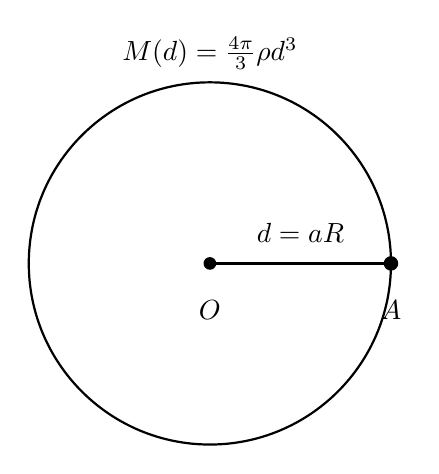
\begin{tikzpicture}[scale=1.15]
\draw[thick] (0,0) circle (2);
\fill (0,0) circle (0.07);
\fill (2,0) circle (0.08);
\draw[thick] (0,0) -- (2,0);
\draw (1,0.12) node[above] {\(d=aR\)};
\draw (0,-0.3) node[below] {\(O\)};
\draw (2,-0.3) node[below] {\(A\)};
\draw (0,2.32) node {\(M(d)=\frac{4\pi}{3}\rho d^3\)};
\end{tikzpicture}\caption{Réduction newtonienne. Pour calculer l’accélération de la galaxie \(A\), les coquilles extérieures se compensent et la masse contenue à l’intérieur du rayon \(d\) agit comme si elle était concentrée en \(O\).}\label{fig:c01-newton-sphere}\end{figure}

Pour une distribution de masse à symétrie sphérique, la force résultante exercée par la matière située à l’extérieur de la sphère passant par \(A\) est nulle. La matière intérieure agit comme si elle était concentrée au centre. La masse enfermée vaut
\begin{equation}
M(d)=\frac{4\pi}{3}\rho d^3.
\label{eq:c01-enclosed-mass}
\end{equation}
La loi de Newton en inverse du carré donne alors l’accélération de \(A\) :
\begin{equation}
\ddot d=-\frac{GM(d)}{d^2}.
\end{equation}
En utilisant l’équation~\eqref{eq:c01-radial-kinematics},
\begin{align}
\ddot a R
&=-\frac{G}{d^2}\left(\frac{4\pi}{3}\rho d^3\right) \\
&=-\frac{4\pi G}{3}\rho d \\
&=-\frac{4\pi G}{3}\rho aR.
\end{align}
le rayon comobile se simplifie, ce qui donne
\begin{equation}
\boxed{\frac{\ddot a}{a}=-\frac{4\pi G}{3}\rho.}
\label{eq:c01-acceleration}
\end{equation}
Cette simplification vérifie la cohérence du modèle. Toute galaxie comobile, quelle que soit sa valeur de \(R\), obéit à la même équation pour un même facteur d’échelle.

En substituant l’équation~\eqref{eq:c01-density-dilution}, on obtient l’une ou l’autre des formes équivalentes suivantes :
\begin{equation}
\frac{\ddot a}{a}=-\frac{4\pi G\nu}{3a^3},
\qquad
\ddot a=-\frac{4\pi G\nu}{3a^2}.
\label{eq:c01-acceleration-nu}
\end{equation}
La première forme fait apparaître l’accélération relative ; la seconde isole \(\ddot a\). Garder \(a\) à gauche est une convention, et ne modifie pas la physique.

\begin{classroomqa}
\audiencequestion{L’origine était arbitraire, pourtant toutes les forces du calcul pointent vers elle. Comment un autre choix d’origine peut-il donner le même Univers ?}
\lecturerresponse{L’équation porte sur le mouvement relatif. En répétant le calcul autour de toute autre galaxie, on obtient la même équation, car l’homogénéité fait dépendre la masse enfermée uniquement du rayon physique. Si l’on passe à un référentiel accéléré lié à une autre galaxie tout en conservant les forces rapportées à la première origine, il faut aussi inclure la force d’inertie correspondante. Choisir un référentiel au repos au centre évite simplement ce calcul supplémentaire. Le résultat invariant est l’équation~\eqref{eq:c01-acceleration}, et non l’existence d’un centre privilégié. \lecturetimestamp{00:43:56--00:46:58}}
\end{classroomqa}

\begin{classroomqa}
\audiencequestion{Le résultat resterait-il valable si la masse comobile par unité de volume \(\nu\) variait d’un lieu à l’autre ?}
\lecturerresponse{Pas sous cette forme à fonction unique. La simplification nette repose sur \(M\propto d^3\) avec la même proportionnalité partout. Si \(\nu\) variait sensiblement sur l’échelle de moyennage, différentes régions nécessiteraient des dynamiques locales différentes et un unique facteur d’échelle homogène ne suffirait plus à les décrire. L’homogénéité joue un rôle essentiel. \lecturetimestamp{00:47:05--00:47:51}}
\end{classroomqa}

\begin{classroomqa}
\audiencequestion{Pourquoi écrire \(\ddot a/a\) au lieu de déplacer le facteur \(a\) à droite ?}
\lecturerresponse{Les deux formes sont correctes. En cosmologie, on écrit conventionnellement l’accélération relative \(\ddot a/a\), en partie parce qu’elle peut être comparée directement au taux d’expansion relatif \(H=\dot a/a\). En multipliant par \(a\), on retrouve la même équation différentielle. \lecturetimestamp{00:50:36--00:51:29}}
\end{classroomqa}

L’équation~\eqref{eq:c01-acceleration} exclut immédiatement un Univers newtonien homogène statique rempli de matière ordinaire. Un facteur d’échelle statique impliquerait \(\ddot a=0\), alors qu’une densité positive rend le membre de droite négatif. Cela ne nous dit \emph{pas} encore si l’Univers est en expansion ou en contraction. Cela indique uniquement le signe de l’accélération.

\section{Une accélération négative n’est pas une contraction}

La distinction entre vitesse et accélération est élémentaire, mais décisive. Une Ferrari qui avance sur l’autoroute peut avoir une vitesse positive tout en freinant, donc avec une accélération négative. De même, un Univers peut avoir
\begin{equation}
\dot a>0,
\qquad
\ddot a<0:
\end{equation}
il est en expansion, mais celle-ci ralentit.

Pour déterminer si le mouvement finira par s’inverser, comparons le problème cosmologique à celui d’une particule test se déplaçant radialement dans le champ gravitationnel de la Terre. Notons maintenant \(x\) la distance physique de la particule à une masse centrale \(M\) ; cette coordonnée n’a aucun rapport avec la coordonnée comobile utilisée précédemment. L’équation de Newton est
\begin{equation}
\ddot x=-\frac{GM}{x^2}.
\label{eq:c01-particle-force}
\end{equation}
L’accélération est toujours dirigée vers l’intérieur. Une particule lancée vers l’extérieur peut néanmoins continuer à s’éloigner longtemps, voire indéfiniment. Une particule déjà en mouvement vers l’intérieur acquiert une vitesse de plus en plus négative. La loi de force ne détermine pas à elle seule le mouvement qui se produit : ce sont les conditions initiales qui en décident.

\begin{classroomqa}
\audiencequestion{Est-ce que \(\ddot a<0\) signifie que l’Univers est en contraction ?}
\lecturerresponse{Non. Une contraction signifie que \(\dot a<0\). Une valeur négative de \(\ddot a\) signifie seulement que \(\dot a\) diminue avec le temps. Si \(\dot a\) est initialement positive, la gravité ralentit l’expansion ; le fait qu’elle atteigne ou non zéro dépend de la vitesse d’expansion initiale, exactement comme le sort d’un projectile lancé vers l’extérieur dépend du fait que sa vitesse soit inférieure ou supérieure à la vitesse de libération. \lecturetimestamp{00:51:30--00:56:18}}
\end{classroomqa}

\begin{figure}[ht]\centering
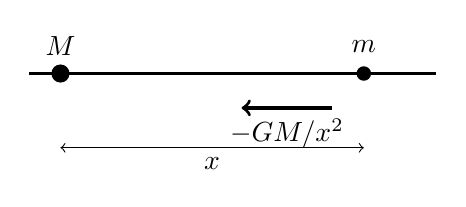
\begin{tikzpicture}[scale=1.15]
\fill (0,0) circle (0.1);
\draw (0,0.3) node {\(M\)};
\draw[thick] (-0.35,0) -- (4.15,0);
\fill (3.35,0) circle (0.08);
\draw (3.35,0.3) node {\(m\)};
\draw[->,very thick] (3.0,-0.38) -- (2.0,-0.38)
  node[midway,below] {\(-GM/x^2\)};
\draw[<->] (0,-0.82) -- (3.35,-0.82)
  node[midway,below] {\(x\)};
\end{tikzpicture}\caption{Le problème radial à une particule qui a permis de distinguer le signe de l’accélération de la direction et du devenir du mouvement.}\label{fig:c01-particle-sketch}\end{figure}

L’énergie rend les différentes possibilités évidentes. L’énergie mécanique conservée est
\begin{equation}
E=\frac12 m\dot x^{\,2}-\frac{GMm}{x}.
\label{eq:c01-particle-energy}
\end{equation}
L’énergie potentielle est proportionnelle à \(1/x\), et non à \(1/x^2\) ; la dérivation de \(-GMm/x\) donne la force en inverse du carré.

\begin{figure}[ht]\centering
\includegraphics[width=0.82\textwidth]{lecture_01_figure_02.png}\caption{Le tableau au début du raisonnement énergétique : une masse test en mouvement et son terme cinétique, juste avant le rétablissement de l’énergie potentielle gravitationnelle.}\lectureframe{00:58:57}\end{figure}

Si \(E<0\), une particule se déplaçant vers l’extérieur ne peut atteindre l’infini, où son énergie potentielle tend vers zéro et son énergie cinétique est non négative. Elle doit s’arrêter à une valeur finie de \(x\), puis revenir. Si \(E>0\), elle ne peut pas s’arrêter, car, à un point de rebroussement, l’énergie cinétique serait nulle et l’énergie potentielle restante serait négative, ce qui contredirait la conservation d’une énergie \(E\) positive. La limite est définie par
\begin{equation}
E=0,
\end{equation}
ce qui définit la vitesse de libération :
\begin{equation}
\frac12 m v_{\rm esc}^2-\frac{GMm}{x}=0,
\qquad
\boxed{v_{\rm esc}^2=\frac{2GM}{x}.}
\label{eq:c01-escape-velocity}
\end{equation}

\begin{figure}[ht]\centering
\includegraphics[width=0.88\textwidth]{lecture_01_figure_03.png}\caption{La limite d’énergie nulle prend forme au tableau. Les équations cosmologiques de l’accélération établies précédemment restent encadrées à gauche, tandis que le problème radial de la vitesse de libération est développé à droite.}\lectureframe{01:01:37}\end{figure}

Exactement à la vitesse de libération, la particule ralentit indéfiniment. Sa vitesse ne tend vers zéro que lorsque \(x\to\infty\) ; elle n’atteint aucun point de rebroussement à distance finie. Ce cas limite sera le modèle cosmologique le plus simple.

\section{L’équation cosmologique de l’énergie}

Revenons à une galaxie située à un rayon comobile fixe \(R\). D’après le théorème des coquilles, son mouvement radial est identique à celui d’une particule qui se déplace à l’extérieur d’une masse ponctuelle égale à la masse enfermée dans sa sphère comobile.

\begin{figure}[ht]\centering
\includegraphics[width=0.82\textwidth]{lecture_01_figure_04.png}\caption{Le croquis de la force en inverse du carré et de la particule radiale, utilisé pour transposer à la cosmologie le raisonnement énergétique à une particule.}\lectureframe{01:04:14}\end{figure}

La masse enfermée n’augmente pas lorsque la sphère physique se dilate. La sphère est comobile et contient donc toujours les mêmes galaxies :
\begin{align}
M
&=\frac{4\pi}{3}\rho(aR)^3 \\
&=\frac{4\pi}{3}\frac{\nu}{a^3}a^3R^3 \\
&=\frac{4\pi}{3}\nu R^3.
\label{eq:c01-fixed-enclosed-mass}
\end{align}
La première expression ne semble dépendre du temps que tant qu’on ne tient pas compte de la dilution de la densité. Les facteurs \(a^3\) se simplifient.

\begin{classroomqa}
\audiencequestion{À mesure que la sphère se dilate, enferme-t-elle davantage de masse ?}
\lecturerresponse{Non. Son rayon physique augmente, mais sa frontière comobile se déplace avec les galaxies. Dans l’écoulement homogène idéal, aucune matière ne traverse cette frontière, et l’équation~\eqref{eq:c01-fixed-enclosed-mass} montre explicitement la simplification. \lecturetimestamp{01:04:37--01:05:20}}
\end{classroomqa}

La vitesse physique de la galaxie est \(\dot d=\dot a R\) et sa distance à l’origine choisie est \(d=aR\). Son énergie newtonienne conservée est donc
\begin{equation}
\boxed{
E=\frac12 m\dot a^{\,2}R^2-\frac{GMm}{aR}.
}
\label{eq:c01-cosmological-energy}
\end{equation}

\begin{figure}[ht]\centering
\includegraphics[width=0.82\textwidth]{lecture_01_figure_05.png}\caption{Les termes cinétique et potentiel cosmologiques au tableau. Le dénominateur complet \(aR\) de l’équation~\eqref{eq:c01-cosmological-energy} découle du rayon physique et de la dérivation qui l’accompagne.}\lectureframe{01:06:12}\end{figure}

Les trois cas de l’énergie d’une particule correspondent à trois cas cosmologiques :
\begin{description}[style=nextline]
\item[\(E<0\) :] l’expansion initiale est inférieure à la vitesse de libération ; \(a(t)\) atteint un maximum, puis l’Univers se recontracte.
\item[\(E=0\) :] l’Univers est exactement critique ; l’expansion ralentit indéfiniment et la vitesse ne tend asymptotiquement vers zéro.
\item[\(E>0\) :] l’expansion initiale est supérieure à la vitesse de libération ; dans le modèle newtonien, l’Univers s’étend indéfiniment avec une vitesse de récession asymptotique non nulle.
\end{description}

Commençons par le cas limite \(E=0\). Posons l’équation~\eqref{eq:c01-cosmological-energy} égale à zéro, simplifions \(m\) et divisons par \(a^2R^2/2\), ce qui donne
\begin{align}
\frac12\dot a^{\,2}R^2&=\frac{GM}{aR}, \\
\left(\frac{\dot a}{a}\right)^2&=\frac{2GM}{a^3R^3}.
\label{eq:c01-energy-intermediate}
\end{align}
Puisque
\begin{equation}
\rho=\frac{M}{(4\pi/3)a^3R^3},
\end{equation}
l’équation~\eqref{eq:c01-energy-intermediate} devient
\begin{equation}
\boxed{
H^2=\left(\frac{\dot a}{a}\right)^2=\frac{8\pi G}{3}\rho.
}
\label{eq:c01-first-friedmann}
\end{equation}
C’est la première équation de Friedmann pour un Univers spatialement plat, composé uniquement de matière et avec une constante cosmologique nulle, obtenue ici par conservation de l’énergie newtonienne.

\begin{classroomqa}
\classquestion{Que se passe-t-il pour une particule lancée exactement à la vitesse de libération ?}
\lecturerresponse{Elle ralentit sans jamais repartir en sens inverse. Sa vitesse ne tend vers zéro qu’à distance infinie. L’Univers d’énergie nulle se comporte de la même façon : \(H\) diminue, mais \(\dot a\) reste positif et aucun retournement ne se produit en un temps fini. \lecturetimestamp{01:10:45--01:12:10}}
\end{classroomqa}

Les facteurs \(4\pi/3\) et \(8\pi G/3\) ne sont pas des éléments décoratifs arbitraires. Le facteur \(4\pi/3\) correspond au volume d’une sphère, et le facteur deux provient de l’énergie cinétique. En relativité générale, le même facteur \(8\pi G\) apparaît dans l’équation de champ d’Einstein, et sa composante temps-temps conduit à l’équation de Friedmann relativiste. Cette concordance n’est pas fortuite, mais la dérivation présentée ici ne prend pas encore en compte la pression, la courbure spatiale en tant que géométrie, ni une constante cosmologique.

\section{La solution critique dominée par la matière}

Utilisons la loi de densité \(\rho=\nu/a^3\) dans l’équation~\eqref{eq:c01-first-friedmann} :
\begin{equation}
\left(\frac{\dot a}{a}\right)^2=\frac{8\pi G\nu}{3a^3}.
\label{eq:c01-matter-friedmann}
\end{equation}
La constante \(\nu\) dépend de la normalisation arbitraire des coordonnées comobiles. Pour faire apparaître la dépendance temporelle, définissons
\begin{equation}
K\equiv\frac{8\pi G\nu}{3}>0.
\end{equation}
Alors
\begin{equation}
\dot a^{\,2}=\frac{K}{a}.
\label{eq:c01-normalized-friedmann}
\end{equation}

\begin{figure}[ht]\centering
\includegraphics[width=0.76\textwidth]{lecture_01_figure_06.png}\caption{La loi de Friedmann dominée par la matière au tableau, d’abord avec ses constantes, puis en mettant en évidence la puissance essentielle inverse du facteur d’échelle.}\lectureframe{01:14:44}\end{figure}

Le membre de droite de l’équation~\eqref{eq:c01-normalized-friedmann} est positif pour toute valeur finie et positive de \(a\). Un retournement exigerait \(\dot a=0\) ; l’Univers critique ne se retourne donc jamais. Son expansion perd peu à peu de sa vigueur, sans toutefois ralentir jusqu’à l’arrêt.

Résolvons maintenant l’équation. On peut séparer directement les variables,
\begin{equation}
a^{1/2}\,da=\sqrt{K}\,dt,
\end{equation}
ou suivre le cours et essayer une loi de puissance,
\begin{equation}
a(t)=Ct^p.
\label{eq:c01-power-trial}
\end{equation}
On a alors
\begin{equation}
\frac{\dot a}{a}=\frac{p}{t},
\qquad
\frac{K}{a^3}=\frac{K}{C^3t^{3p}}.
\end{equation}
La substitution dans l’équation~\eqref{eq:c01-matter-friedmann} donne
\begin{equation}
\frac{p^2}{t^2}=\frac{K}{C^3t^{3p}}.
\end{equation}
L’identification des puissances et des coefficients donne
\begin{equation}
3p=2,
\qquad
C^3=\frac{K}{p^2}=\frac{9K}{4}.
\end{equation}
Ainsi,
\begin{equation}
\boxed{
a(t)=\left(\frac{3\sqrt K}{2}t\right)^{2/3}\propto t^{2/3}.
}
\label{eq:c01-two-thirds}
\end{equation}
L’origine additive du temps a été choisie de sorte que \(a=0\) à \(t=0\). Plus généralement, on peut remplacer \(t\) par \(t-t_0\).

Le facteur d’échelle croît indéfiniment, tandis que
\begin{equation}
\dot a\propto t^{-1/3}\longrightarrow0,
\qquad
H=\frac{2}{3t}\longrightarrow0.
\label{eq:c01-asymptotic-slope}
\end{equation}
Sa courbe est toujours croissante et toujours concave vers le bas. Elle ne tend vers aucune droite horizontale, car \(a(t)\) n’est pas borné, mais sa pente tend vers zéro.

\begin{classroomqa}
\audiencequestion{A-t-on obtenu \(t^{2/3}\) uniquement parce que cette forme d’essai a fonctionné ? Un autre essai pourrait-il donner une autre solution d’énergie nulle ?}
\lecturerresponse{L’essai permet d’identifier la solution, et pas simplement une possibilité. L’équation du premier ordre pour la branche en expansion \(\dot a=\sqrt{K/a}\) s’intègre de façon unique, à la normalisation et au choix de l’origine des temps près, en \(a\propto(t-t_0)^{2/3}\). Des énergies totales différentes donnent des équations différentielles différentes, et donc des histoires cosmologiques différentes. \lecturetimestamp{01:27:07--01:27:43}}
\end{classroomqa}

\begin{classroomqa}
\audiencequestion{La courbe critique finit-elle par devenir horizontale ?}
\lecturerresponse{Sa pente tend vers zéro : \(\dot a\propto t^{-1/3}\). Elle reste néanmoins positive à tout instant fini, de sorte que le facteur d’échelle continue de croître sans borne. L’Univers tend asymptotiquement vers le repos sans jamais l’atteindre. \lecturetimestamp{01:27:48--01:28:57}}
\end{classroomqa}

Ce résultat simple est historiquement frappant. Newton possédait la mécanique et le théorème des coquilles nécessaires à cette dérivation, et il s’est intéressé à des questions concernant un Univers gravitant infini, mais il n’a pas formulé le modèle en expansion. La discussion en cours a suggéré que ses engagements philosophiques et théologiques concernant l’histoire cosmique ont peut-être influencé les questions qui lui semblaient naturelles. Cette suggestion historique ne fait pas partie de la dérivation ; le seul point mathématique est que les outils newtoniens requis existaient déjà.

\begin{classroomqa}
\audiencequestion{Cette construction newtonienne suppose-t-elle un Univers infini ?}
\lecturerresponse{Elle suppose un espace newtonien euclidien et spatialement plat. Dans le modèle newtonien usuel, cet espace s’étend indéfiniment : le modèle est donc spatialement infini, même si les distances entre galaxies comobiles changent au cours du temps. Les géométries spatiales courbes et finies relèvent du traitement relativiste. \lecturetimestamp{01:22:12--01:22:55}}
\end{classroomqa}

\section{Au-delà du modèle d’énergie nulle}

Le cas d’énergie nulle est une simplification délibérée, et non le seul Univers newtonien possible. En conservant \(E\neq0\) dans l’équation~\eqref{eq:c01-cosmological-energy}, on obtient
\begin{equation}
\left(\frac{\dot a}{a}\right)^2
=\frac{8\pi G}{3}\rho+\frac{2E}{mR^2a^2}.
\label{eq:c01-nonzero-energy}
\end{equation}
L’homogénéité exige que la combinaison \(2E/(mR^2)\) soit la même pour toute sphère comobile représentative. En la notant \(C_E\),
\begin{equation}
H^2=\frac{8\pi G}{3}\rho+\frac{C_E}{a^2}.
\end{equation}
Une valeur positive de \(C_E\) correspond à une énergie supérieure à celle de libération ; une valeur négative de \(C_E\) permet un retournement. En notation relativiste, ce terme d’énergie est réinterprété en termes de courbure spatiale, un lien que nous réserverons à la suite.

Les trois évolutions où seule la matière domine ont une accélération négative :
\begin{equation}
\ddot a=-\frac{4\pi G}{3}\rho a<0.
\end{equation}
La courbe de recollapse monte, atteint \(\dot a=0\), puis redescend. La courbe critique \(t^{2/3}\) monte indéfiniment, avec une pente qui tend vers zéro. La courbe d’énergie positive monte elle aussi indéfiniment et tend vers une croissance linéaire. Un premier schéma provisoire au tableau de ces cas a été corrigé pendant le cours ; la conclusion qui demeure est leur comportement commun, concave vers le bas, et non chaque détail du premier schéma.

L’Univers observé présente un phénomène supplémentaire. Son expansion initiale, dominée par la matière, est bien approchée par une courbe décélérée, mais aux temps tardifs, la courbe se redresse vers le haut :
\begin{equation}
\ddot a>0.
\end{equation}
La matière ordinaire sans pression ne peut produire ce signe dans l’équation~\eqref{eq:c01-acceleration}. Un terme supplémentaire est nécessaire. Dans le modèle moderne le plus simple, il s’agit d’une constante cosmologique ; plus généralement, on parle d’énergie noire. Ce chapitre l’omet délibérément afin de commencer par étudier clairement la dynamique newtonienne de la matière.

\begin{classroomqa}
\audiencequestion{Le \(8\pi G\) de l’équation de Friedmann est-il le même facteur que celui qui apparaît dans l’équation de champ d’Einstein, et avons-nous inclus une constante cosmologique ?}
\lecturerresponse{La même normalisation gravitationnelle apparaît en relativité générale, et l’équation de champ correspondant à la composante temps-temps reproduit l’équation de Friedmann relativiste. Le modèle considéré ici ne contient pas de constante cosmologique. C’est un univers dominé par la matière ; le terme de constante cosmologique manquant est précisément le type de terme qui peut rendre compte de l’accélération aux temps tardifs. \lecturetimestamp{01:30:15--01:31:06}}
\end{classroomqa}

\section{Le mouvement moyen et les écarts locaux}

L’expansion homogène est une description à gros grain. Cela ne signifie pas que chaque objet s’éloigne de tous ses voisins proches. Les systèmes liés par la gravitation ou autrement peuvent se découpler du flot de Hubble. La Voie lactée et Andromède, par exemple, se rapprochent au lieu de suivre la loi de récession à grande échelle.

L’écart entre la vitesse d’une galaxie donnée et le flot de Hubble est appelé sa \emph{vitesse particulière}. C’est un terme technique, qui ne porte aucun jugement sur la galaxie. La loi de Hubble constitue une meilleure approximation lorsqu’on fait la moyenne sur des distances et des volumes plus grands. À l’échelle d’une galaxie liée, d’un amas ou d’une région localement surdense, les forces locales peuvent dominer l’expansion de fond.

\begin{classroomqa}
\audiencequestion{Certaines régions peuvent-elles se contracter alors même que l’Univers est globalement en expansion ?}
\lecturerresponse{Bien sûr. Les systèmes liés et les fluctuations suffisamment denses ne sont pas tenus de suivre l’expansion moyenne. Le système Voie lactée--Andromède en est un exemple familier. Un calcul cosmologique fait la moyenne sur des volumes suffisamment grands pour que ces mouvements particuliers et les fluctuations locales de densité ne dominent pas ; le \(a(t)\) qui en résulte décrit le fond cosmologique, et non chaque paire d’objets. \lecturetimestamp{01:31:00--01:34:13}}
\end{classroomqa}

L’analogie est celle d’un gaz ordinaire. Qualifier l’air d’une pièce d’uniforme ne revient pas à nier les fluctuations moléculaires ni les variations locales de densité. Cela signifie que les moyennes calculées sur des régions suffisamment grandes sont stables. L’homogénéité cosmique a le même statut logique, quoique sur des échelles immensément plus grandes. Une région initialement légèrement plus dense que la moyenne peut avoir une auto-gravité suffisante pour résister à l’expansion et finir par s’effondrer en une structure liée.

\begin{classroomqa}
\audiencequestion{Les observations permettent-elles de déterminer si les galaxies se déplacent dans l’espace ou si l’expansion de l’espace les entraîne en les éloignant les unes des autres ?}
\lecturerresponse{Pas lorsque les deux descriptions attribuent la même distance \(d_{AB}(t)\) à chaque paire. Dans l’une, les galaxies se déplacent sur un arrière-plan de coordonnées qui semble fixe ; dans la description comobile, les galaxies restent fixes et le facteur d’échelle rend compte du changement. Ces descriptions sont mathématiquement équivalentes. La relativité générale rend le second langage plus naturel, mais cette comparaison ne fait apparaître aucun observable distinct. \lecturetimestamp{01:34:14--01:34:59}}
\end{classroomqa}

\begin{classroomqa}
\audiencequestion{Outre la luminosité des supernovæ de type Ia, existe-t-il des indices indépendants de l’accélération cosmique ?}
\lecturerresponse{Oui. Cette inférence s’appuie sur un ensemble d’observations, en particulier sur la façon dont les mesures des supernovæ et le fond diffus cosmologique concordent. Aucune donnée isolée ne suffit à elle seule à établir cette conclusion ; l’essentiel est la cohérence entre des mesures cosmologiques indépendantes. \lecturetimestamp{01:35:00--01:35:38}}
\end{classroomqa}

\section{Ce qui a été établi}

Le raisonnement a suivi un ordre rigoureux :
\begin{enumerate}
\item L’isotropie à grande échelle, conjuguée au rejet d’un centre privilégié, motive l’homogénéité.
\item L’homogénéité permet d’introduire un réseau comobile doté d’un unique facteur d’échelle \(a(t)\).
\item La dérivation de la distance physique donne la loi de Hubble,
  \[
  H=\frac{\dot a}{a},
  \qquad
  v=Hd.
  \]
\item La conservation de la masse dans une cellule comobile donne
  \[
  \rho=\frac{\nu}{a^3}.
  \]
\item Le théorème des coquilles de Newton donne l’équation d’accélération
  \[
  \frac{\ddot a}{a}=-\frac{4\pi G}{3}\rho.
  \]
\item La conservation de l’énergie permet de distinguer les cas d’une expansion suivie d’une recontraction, d’une expansion critique et d’une expansion non liée.
\item À énergie totale nulle,
  \[
  H^2=\frac{8\pi G}{3}\rho,
  \qquad
  a(t)\propto t^{2/3}.
  \]
\end{enumerate}

Il s’agit d’un modèle newtonien complet dominé par la matière, mais pas encore d’une description complète de notre Univers. Il rend compte de la dynamique initiale de décélération, montre pourquoi un univers homogène rempli de matière ne peut rester statique et identifie l’expansion critique à la limite de l’échappement. L’énergie non nulle, la géométrie spatiale relativiste, la pression, le rayonnement et le terme responsable de l’accélération tardive restent à ajouter.
